\documentclass[%
	11pt,
	a4paper,
	utf8,
	%twocolumn
		]{article}	

\usepackage{style_packages/podvoyskiy_article_extended}


\begin{document}
\title{Общие и специальные вопросы оптимизации}

\author{\itshape Подвойский А.О.}

\date{}
\maketitle

\thispagestyle{fancy}

%Здесь приводятся заметки по специальным вопросам теории оптимизации


\shorttableofcontents{Краткое содержание}{1}

\tableofcontents

\section{Полезные ссылки}

\url{https://github.com/ceandrade/brkga_mip_feasibility}

\section{Методы решения задач линейного программирования}

Задачи линейного программирования относятся к подклассу задач выпуклого программирования \cite[\strbook{57}]{vorontsova:convex_opt-2021}.

\subsection{Симплекс-метод Данцига}

\remark{
	В худшем случае симплекс-метод работает за экспоненциальное время, но в целом на практике обычно он работает очень быстро, и многочисленные эксперименты и исследования метода подтвердили полиномиальное время работы \cite[\strbook{61}]{vorontsova:convex_opt-2021}
}

Для оценки вычислительной сложности симплекс-метода Данцига Спилман и Тенг предложили использовать \emph{сглаженный анализ}. Сглаженный анализ -- вероятностный анализ алгоритма, при котором изучается работа алгоритма при незначительном случайном возмущеннии конкретных входных данных, а затем ищется зависимость производительности алгоритма от размера входа и от среднеквадратичного отклоненеия возмощений.

Так вот Спилман и Тенг показали, что симплекс-метод имеет \emph{\underline{полиномиальную} сглаженную сложность}\footnote{В том же 2006 году оценка симплекс-метода Спилмана и Тенга была улучшена. Р. Вершининым. Он показал, что ожидаемое время работы симплекс-метода на незначительно измененных входных данных является полиномом от логарифма количества ограничений $ n $}. Эти результаты означают, что хотя и существуют задачи, на которых симплекс-метод будет работать \emph{экспоненциально} долго, но если исходные данные таких задач (коэффициенты целевой функции и ограничений) подвергнуть незначительному изменению, то с достаточно высокой вероятностью симплекс-метод на возмущенной задаче уже будет работать за \emph{полиномиальное время} \cite[\strbook{62}]{vorontsova:convex_opt-2021}.

В конце 1970-х годов обнаружили, что алгоритмы, в общем случае решающие задачи линейного программирования за полиномиальное время, все-таки существуют. Все такие полиномиальные алгоритмы -- \emph{методы внутренней точки} (первый метод внутреней точки с полиномиальной сложностью -- метод Кармаркара) и \emph{метод эллипсоидов} -- отличались от симплекс-метода геометрическим подходом.

В течение 50 лет оставался открытым вопрос, существует ли полиномиальный алгоритм, который работает подобно симплекс-методу, перебирая только вершины (угловые точки) допустимого множества задачи. Ответ на этот вопрос дали Келнер и Спилман в 2006 году: они представили \underline{рандомизированный} симплекс-метод с \emph{полиномиальным временем работы}.

\remark{%
В современных оптимизационных пакетах задачи линейного программирования средней размерности (вплоть до сотен тысяч и даже миллиона переменных или ограничений) решаются \underline{\itshape методами внутренней точки}.
}

Постановка задачи. Найти максимум функции
\begin{align*}
f(x) = \sum_{j=1}^{n} c_j x_j \leftarrow c^T x
\end{align*}
при ограничениях
\begin{align*}
	\sum_{j=1}^{n} a_{ij} x_j = b_i, \ i = 1, \ldots, m\  (m < n) \leftarrow Ax = b,\\
	x_j \geqslant 0, \ j = 1, \ldots, n.
\end{align*}

Такая постановка называется \emph{канонической}, а искомое решение $ x^{*} = (x_1^{*}, \ldots, x_n^{*})^T $ -- \emph{оптимальным}.

Замечания:
\begin{itemize}
	\item Максимизируемая функция и ограничения \underline{линейны} по $ x_j, \ j = 1, \ldots, n $,
	
	\item Задача содержит ограничения на неотрицательность переменных, присутствие которых диктуется процедурой симплекс-метода. Если по физической постановке задачи какая-либо переменная, например, $ x_n $, неограничена по знаку, то ее можно представить в виде $ x_n = x_{n+1} - x_{n+2} $, где $ x_{n+1}, x_{n+2} \geqslant 0 $,
	
	\item В ограничениях $ \sum\limits_{j=1}^{n} a_{ij} x_j = b_i, \ i = 1, \ldots, m\  (m < n) $ будем считать переменные $ b_i \geqslant 0, \ i = 1, \ldots, m $.
\end{itemize}

Стратегия метода Данцига решения описаной задачи основана на особенностях постановки этой задачи. Множество
\begin{align*}
	X = \{ x \, | \, \sum_{i}^{n} a_{ij} x_j = b_i, \ i = 1, \ldots, m, \ x \in \mathbb{R}^n, \ x_j \geqslant 0, \ j = 1, \ldots, n \}
\end{align*}
допустимых решений задачи -- есть выпуклое множество, которое геометрически представляет собой \emph{выпуклый политоп}\footnote{Политоп -- подмножество Евклидова пространства, представимое объединением симплексов ($ n $-мерное обобщение треугольника)}, имеющий конечное число \emph{крайних точек}.

\emph{Крайней точкой выпуклого множества} $ X $ называется точка $ x \in X $, которая не может быть выражена в виде выпуклой комбинации других точек $ y \in X, x \neq y $.

Стратегия решения задачи симплекс-методом состоит в направленном переборе базисных решений, определяющих крайние точки политопа. Направленность перебора предполагает следующую организацию вычислительного процесса \cite{panteleev}:
\begin{enumerate}
	\item Нахождение базисного решения (метод Гаусса-Жордана, переход к $ M $-задаче),
	
	\item Переход от одного базисного решения к другому таким образом, чтобы обеспечить улучшение целевой функции (другими словами, переход от одной \emph{вершины политопа} к другой в направлении улучшения целевой функции).
\end{enumerate}






\section{Методы решения задач линейного целочисленного программирования}

\subsection{Метод ветвей и границ}

Постановка задачи (Mixed Integer Linear Programming, MILP)
\begin{align*}
	f(x) = \sum_{j=1}^{n} c_j x_j \rightarrow \max
\end{align*}
при ограничениях
\begin{align*}
	\sum_{j=1}^{n} a_{ij} x_j \geqslant b_i, \ i = 1, \ldots, m,\\
	x_j \geqslant 0, \ x \in \mathbb{Z}, \ j = 1, \ldots, n.
\end{align*}

\remark{%
Описанная задача является задачей линейного целочисленного программирования. Ограничения, связанные с целочисленностью, могут быть наложены не на все переменные, а лишь на их часть
}

\textbf{Стратегия поиска}

Для корня дерева ветвей-и-границ (branch-and-bound tree) описанная задача решается \emph{симплекс-методом} \underline{без учета ограничений на целочисленность} (т.е. в релаксированной постановке). Считаеся, что она имеет решение. На полученном оптимальном решении $ x^{0*} = (x_1^{0*}, \ldots, x_n^{0*}) $ вычисляется значение \emph{целевой функции} $ f(x^{0*}) $.

Если решение $ x^{0*} $ является целочисленным, то поставленная задача решена. Если решение $ x^{0*} $ оказывается \underline{нецелочисленным}, то значение $ f(x^{0*}) $ (полученное для решаемой задачи в релаксированной постановке) является \emph{верхней границей} (потому что мы решаем задачу на максимум) возможных оптимальных значений $ f(x) $ на целочисленных решениях.

При нецелочисленном решении дальнейшая процедура решения задачи состоит в ее ветвлении на две подзадачи. Целью этого ветвления является разбиение множества допустимых решений на два подмножества путем построения дополнительных ограничений таким образом, чтобы исключить нецелочисленную точку $ x^{0*} $ и сделать решение по крайней мере одной из задач целочисленным по одной выбранной координате $ x_k $.

Координатой $ x_k $ может быть \cite[\strbook{339}]{panteleev}:
\begin{enumerate}
	\item Нецелочисленная координата с наименьшим или наибольшим индексом.
	
	\item Нецелочисленная координата с наименьшей или наибольшей дробной частью.
	
	\item Нецелочисленная координата, которой соответствует наибольший коэффициент в целевой функции.
	
	\item Нецелочисленная координата, выбранная на основани приоритетов, определяемых физическим содержанием задачи.
\end{enumerate}

Для построения дополнительных ограничений округляем нецелочисленное решение вниз и исследуем область значений левее, т.е. $ x_k \leqslant \floor{x_k^{0*}} $, и округляем вверх и исследуем область правее, т.е. $ \ceil{x_k^{0*}} \leqslant x_k $.

Построение дополнительных ограничений позволило исключить из рассмотрения оптимальное \underline{нецелочисленное} решение $ x^{0*} $ и обеспечить \underline{целочисленность} значений координаты $ x_k $.

\begin{figure}[h]
	\centering
	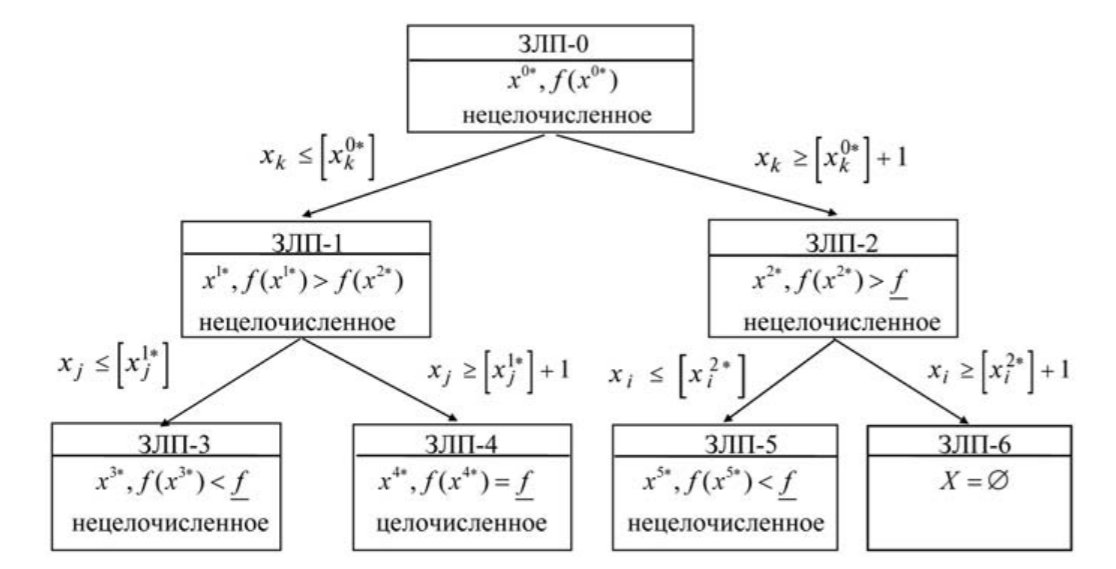
\includegraphics[scale=0.7]{figures/bb_tree.png}
	\caption{ Пример дерева ветвей-и-границ }\label{fig:bb_tree}
\end{figure}

Задачи ЗЛП-1 и ЗЛП-2 записываются в виде, изображенном на \pic{fig:zlp_1_and_zlp_2}.

\begin{figure}[h]
	\centering
	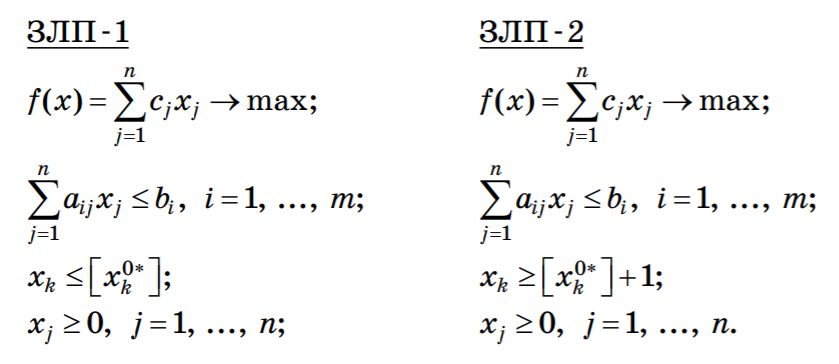
\includegraphics[scale=0.6]{figures/zlp_1_and_zlp_2.png}
	\caption{ Подзадачи корневого узла дерева ветвей-и-границ }\label{fig:zlp_1_and_zlp_2}
\end{figure}

Задачи ЗЛП-1 и ЗЛП-2 решаются самостоятельно симплекс-методом \emph{без учета ограничений на целочисленность} координта $ x_j, \ j = 1, \ldots, n $. Вычисляются значения функции $ f(x) $ на оптимальных решениях обеих задач. Если ни одна из них не имеет целочисленного решения, то выбрирается задача для приоритетного дальнейшего ветвления по установленному правилу: например, приоритетному ветвлению подлежит та задача, в которой значение $ f(x) $ на оптимальном \emph{нецелочисленном} решении максимально.

Пусть $ f(x^{1*}) > f(x^{2*}) $, тогда задача ЗЛП-1 первой ветвится на ЗЛП-3 и ЗЛП-4, которые решаются симплекс-методом \emph{без учета требований на целочисленность} с последующим анализом решений \cite[\strbook{340}]{panteleev}. Если ни одна из задач ЗЛП-3 и ЗЛП-4 не имеет целочисленного решения, приступают к ветвлению задачи ЗЛП-2.

Процесс ветвления продолжается до тех пор, пока не будет получено в одной из ветвей целочисленное решение. Пусть задача ЗЛП-4 имеет целочисленное решение.  Обозначим $ \underline{f} $ -- значение функции на первом целочисленном решении: $ \underline{f} = f(x^{4*}) $. Соответсвующее целочисленное решение включается в множество $ \bar{X}^* $ возможных оптимальных решений исходной задачи.

После того, как найдено первое целочисленное решение, вопрос о дальнейшем ветвлении других задач решается на основании сравнения значений $ f(x^{k*}) $ на оптимальных \underline{нецелочисленных} решениях в оставшихся ветвях со значением $ \underline{f} $.

Если $ f(x^{k*}) \leqslant \underline{f} $ для всех оставшихся $ k $, то расчет закончен. Решениями исходной задачи являются те целочисленные решения $ x^{k*} $, для которых $ f(x^{k*}) = \underline{f} $.

Если $ f(x^{k*}) > \underline{f} $, то соответствующая этому номеру $ k $ задача ветвится далее. Так, на \pic{fig:bb_tree} имеем $ f(x^{2*}) > \underline{f} $ и $ f(x^{3*}) < \underline{f} $. Задача ЗЛП-2 подлежит ветвлению на ЗЛП-5, ЗЛП-6, а задача ЗЛП-3 не подлежит. Задача ЗЛП-6 не имеет решения, так как множество допустимых решений пустое, и далее не рассматривается. Задача ЗЛП-5 имеет нецелочисленное решение $ x^{5*}, f(x^{5*}) $. Если $ f(x^{5*}) < \underline{f} $, то решение задачи закончено и $ x^* = x^{4*}, f(x^*) = \underline{f} $. В противном случае задача ЗЛП-5 ветвится дальше.

Если в одной из задач получено целочисленное решение, то ее ветвление далее не прозводится. Если соответствующее значение целевой функции $ \geqslant \underline{f} $, решение считается принадлежащим множеству $ X^* $ возможных оптимальных решений исходной задачи.

Если значение целевой функции $ < \underline{f} $, целочисленное решение не включается в множество $ X^* $.

Таким образом, ветвление какой-либо задачи заканчивается, если выполняется одно из условий \cite{panteleev}:
\begin{enumerate}
	\item решение целочисленное,
	
	\item значение целевой функции данной задачи $ \leqslant \underline{f} $,
	
	\item множество допустимых решений пустое.
\end{enumerate}

Если ветвление всех задач закончено, то в множестве $ X^* $ выбирается решение (решения), которому соответствует наибольшее значение целевой функции. Оно является решением исходной задачи. Если множество $ X^* $ пустое, то исходная задача не имеет решения.

\subsection{Первичные эвристики в SCIP}

Алгоритм ветвей-и-границ представляет собой \emph{полную} (complete) процедуру. Это означает, что алгоритм гарантирует оптимальное решение каждой проблемы за конечное время. Однако, это очень дорогой в вычислительном смысле метод и в худшем случае временные издержки будут экспоненйиально зависеть от размерности задачи.

В противоположенность первичные эвристики относятся к \emph{неполным} (incomplete) методам. То есть они пытаются найти допустимое решение приемлемого качества за небольшой промежуток времени. Но они не гарантируют оптимальности решения.

Первичные эвристики в SCIP условно могут быть разделены на 4 категории \cite{achterberg:constr_int_prog}:
\begin{itemize}
	\item Эвристики округления (rounding heuristics) пытаются округлять значения переменных релаксированного решения таким образом, чтобы полученное округленное решение оставалось допустимым,
	
	\item Глубокие эвристики (diving heurisctics) начинают с текущего релаксированного решения задачи и итеративно фиксируют целочисленные значения целочисленных переменных и решают текующую задачу заново,
	
	\item Целевые глубокие эвристики (objective diving heuristics) похожи на глубокие эвристики, но вместо фиксации переменных, они изменяют значения коэффициентов в целевой функции,
	
	\item Улучшающие эвристики (improvenment heuristics) исследуют одно и несколько допустимых решений и пытаются построить такое решение, которому отвечает более низкое (в случае задачи минимизации) или более высокое (в случае задачи максимизации) значение целевой функции.
\end{itemize}

\subsubsection{Эвристики округления}

\paragraph{RENS} 


\section{Общие положения постановки частично-целочисленного линейного программирования}

Задача линейного программирования в частично-целочисленной постановке (Mixed Integer Linear Program, MILP, MIP) записывается в форме
\begin{align*}
	\min c^T x,\\
	Ax = b,\\
	x \geqslant 0,\\
	x_i \in \mathbb{Z} \quad \forall i \in \mathcal{I}
\end{align*}

Задача, когда все переменные являются целочисленными, называется задачей линейного программирования в чистой целочисленной постановке (Pure Integer Linear Program, ILP, IP).

Если все переменные принимаются значения из множества $ \{ 0, 1 \} $, то задача называется задачей линейного программирования 0-1 (0-1 linear program).

Включение целочисленных переменных в постановку задачи расширяет возможности моделирования.

Задачи линейного программирования могут быть решены за полиномиальное время \emph{методами внутренней точки} (метод эллипсоида, алгоритм Кармаркара). 

Задачи целочисленного программирования относятся к классу NP-трудных:
\begin{itemize}
	\item на текущий момент не известны алгоритмы, способные решить этот такого рода задачи за полиномиальное время,
	
	\item И, вообще говоря, есть мало шансов, что такие алгоритмы когда-нибудь будут найдены.
\end{itemize}

Релаксированное решение можно получить, сняв ограничения на целочисленность
\begin{align*}
	\min c^T x,\\
	Ax = b,\\
	x \geqslant 0.
\end{align*}

\remark{
Задачу линейного программирования в частично-целочисленной постановке нельзя решить, просто перейдя от решения задачи в релаксированной постановке с последующем округлением переменных
}

Например, оптимальным решением задачи линейного программирования в чистой целочисленной постановке будет
\begin{align*}
	\max x + y\\
	-2x + 2 y \geqslant 1,\\
	-8 x + 10 y \leqslant 13,\\
	x,y \geqslant 0,\\
	x,y \in \mathbb{Z}
\end{align*}
вектор $ (x, y) = (1, 2) $, которому отвечает целевая функция со значением 3.

А релаксированным оптимальным решением будет вектор $ (x, y) = (4, 4.5) $ со значением целевой функции 9.5. 

Не существует прямого способа перейти от релаксированного решения к целочисленному.

\begin{figure}[h]
	\centering
	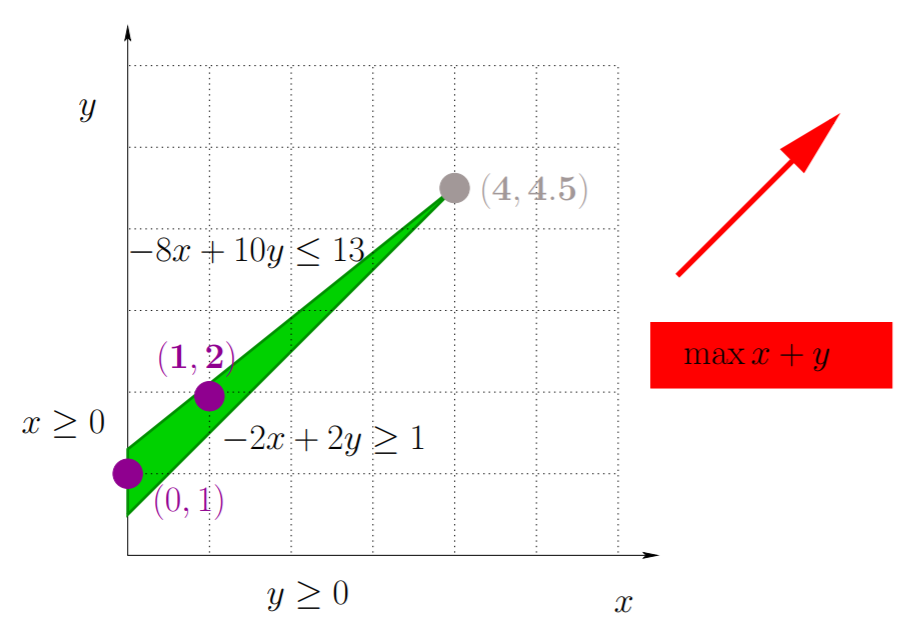
\includegraphics[scale=0.55]{figures/lp_and_mip.png}
	\caption{ Связь релаксированной и целочисленной постановок задачи }\label{fig:lp_and_mip}
\end{figure}

Предполагается, что переменные ограничены, т.е. имеют нижнюю и верхнюю границы.

Через $ P_0 $ обозначим рассматриваемую постановку задачи, а через $ LP(P_0) $ релаксированное решение задачи $ P_0 $. Если в оптимальном релаксированном решении $ LP(P_0) $ все целочисленные переменные принимают целочисленные значения, то это решение будет решением исходной задачи $ P_0 $.

В противном случае для целочисленной переменной $ x_j $, которая принимает нецелочисленное значение $ \beta_j, \ \beta_j \notin \mathbb{Z} $ в оптимальном релаксированном решении $ LP(P_0) $, определяются подзадачи
\begin{align*}
	P_1 := P_0 \wedge x_j \leqslant \floor*{\beta_j},\\
	P_2 := P_0 \wedge x_j \geqslant \ceil*{\beta_j}.
\end{align*}

Тогда физичным решением исходной задачи будет
$$
feasibleSols(P_0) = feasibleSols(P_1) \cup feasibleSols(P_2).
$$



\listoffigures\addcontentsline{toc}{section}{Список иллюстраций}

% Источники в "Газовой промышленности" нумеруются по мере упоминания 
\begin{thebibliography}{99}\addcontentsline{toc}{section}{Список литературы}
	\bibitem{achterberg:constr_int_prog}{\emph{Achterberg T.} Constraint Integer Programming, 2007 }
	
	\bibitem{panteleev}{\emph{Пантлеев А. В., Летова Т.А,} Методы оптимизации в примерах и задачах. -- СПб.: Издательство <<Лань>>, 2015. -- 512 с.}
	
	\bibitem{vorontsova:convex_opt-2021}{\emph{Вороноцова Е.А.} Выпуклая оптимизация. -- М.: МФТИ, 2021. -- 364 с.}
	
	\bibitem{burkov:2020}{\emph{Бурков А.} Машинное обучение без лишних слов. -- СПб.: Питер, 2020. -- 192 с.}
		
	\bibitem{beazley:python-2010}{\emph{Бизли Д.} Python. Подробный справочник. -- Пер. с англ. -- СПб.: Символ-Плюс, 2010. -- 864~с. }
\end{thebibliography}

\end{document}
